\documentclass[11pt,a4paper]{article}
\usepackage[utf8]{inputenc}
\usepackage[T1]{fontenc}
\usepackage[spanish,es-tabla]{babel}
\usepackage{amsmath,amssymb}
\usepackage{graphicx}
\usepackage{geometry}
\usepackage{listings}
\usepackage{xcolor}
\usepackage{hyperref}
\usepackage{float}
\usepackage{caption}

\geometry{margin=2.5cm}

\definecolor{codegray}{rgb}{0.5,0.5,0.5}
\definecolor{codegreen}{rgb}{0,0.6,0}
\definecolor{backcolour}{rgb}{0.95,0.95,0.92}

\lstdefinestyle{mystyle}{
    backgroundcolor=\color{backcolour},
    commentstyle=\color{codegreen},
    keywordstyle=\color{blue},
    numberstyle=\tiny\color{codegray},
    basicstyle=\ttfamily\footnotesize,
    breakatwhitespace=false,
    breaklines=true,
    captionpos=b,
    keepspaces=true,
    numbers=left,
    numbersep=5pt,
    showspaces=false,
    showstringspaces=false,
    showtabs=false,
    tabsize=2
}
\lstset{style=mystyle}

\graphicspath{{capturas/}{../capturas/}}

\title{\textbf{Reporte de Avances: Corrección de Ruido en la Plataforma HIL\\ para el Control de Péndulo Invertido}}
\author{Ing. Eduardo Pascual Pérez\\Maestría en Robótica -- UTM}
\date{Versión original: 12 de Octubre del 2026\\Actualización: 1 de Noviembre del 2026}

\begin{document}
\maketitle

\section{Introducción}

En las sesiones de trabajo de la presente semana se abordaron los problemas de ruido que se venian presentando en las señales adquiridas por el sistema Hardware-in-the-Loop (HIL) del péndulo invertido. El objetivo principal fue diagnosticar la causa raíz del ruido excesivo observado en la variable de velocidad angular y proponer una solución que no rompiera la naturaleza HIL del sistema, es decir, que todo el lazo de control se mantuviera ejecutandose sobre el microcontrolador TMS320F28379D y no migrara hacia la computadora.

A lo largo de este reporte se detallan los errores que se encontraron en la configuración, las pruebas que se realizaron para diagnosticar cada uno, los cambios aplicados al firmware, los resultados cuantitativos obtenidos, y las pruebas que se omitieron junto con su justificación. Adicionalmente se documenta la comparación cuantitativa del lazo cerrado entre el DSP y una simulación en MATLAB, la cual permitió validar que el algoritmo implementado en el microcontrolador coincide con el modelo teórico hasta el nivel de cuantización del ADC. Finalmente se documenta la verificación del baud rate mediante software de puerto serial y el análisis multi-tasa del lazo de control.

\paragraph{Actualización del 31 de octubre / 1 de noviembre de 2026.} Después de la versión original de este reporte se trabajó sobre el modelo \emph{sin perturbación, un solo núcleo (CPU1)}, cuyo ángulo real se estabilizaba en $\approx 0.014$ rad en lugar de 0 rad. Se encontró que (i) el reloj del sistema estaba a 100 MHz en vez de 200 MHz por falta de un símbolo de compilación, (ii) el offset de la cadena DAC$\rightarrow$ADC dependía de esa configuración y podía calibrarse, (iii) la telemetría se bloqueaba por el uso de \texttt{sprintf}, y (iv) existía un artefacto en la primera muestra. Las secciones nuevas están marcadas en el texto; donde la versión de octubre contenía afirmaciones que resultaron incorrectas o incompletas, se corrigieron y se indica explícitamente.

\section{Antecedentes y arquitectura del sistema}

El sistema HIL que se esta desarrollando consta de las siguientes partes:

\begin{itemize}
    \item \textbf{Firmware en el DSP:} se ejecuta un controlador PID y la simulación de la planta (péndulo invertido linealizado) mediante el método de Euler hacia adelante. La simulación corre a un periodo de $T_s = 10\,\mu s$ dentro de una interrupción del temporizador.
    \item \textbf{Middleware en Python:} recibe las tramas del DSP por UART, las decodifica, guarda un archivo CSV y actualiza el gemelo digital en CoppeliaSim.
    \item \textbf{CoppeliaSim:} actua como gemelo digital cinemático, mostrando visualmente el estado del péndulo.
    \item \textbf{MATLAB:} se utiliza para el post-procesamiento de los datos guardados y para la simulación del lazo cerrado.
\end{itemize}

El DSP envia cada 10 ms (100 Hz) una trama con tres valores separados por comas: posición, velocidad y acción de control, todos escalados por un factor de 1000 para enviarlos como enteros y aprovechar mejor el canal UART.

\subsection{Arquitectura multi-tasa del lazo de control}

Un aspecto crítico del sistema es su naturaleza \textbf{multi-tasa}. Conviven tres frecuencias distintas de operación:

\begin{table}[H]
\centering
\caption{Tasas de operación del sistema HIL}
\begin{tabular}{lccc}
\hline
\textbf{Tarea} & \textbf{Frecuencia} & \textbf{Período} & \textbf{Ejecutor} \\
\hline
Integración de planta + PID & 100 kHz & 10 $\mu$s & ISR del DSP \\
Cálculo de derivada lenta & 100 Hz & 10 ms & ISR (cada 1000 ejecuciones) \\
Reporte UART & 100 Hz & 10 ms & Bucle principal del DSP \\
Post-procesamiento & 100 Hz & 10 ms & Python + MATLAB \\
\hline
\end{tabular}
\end{table}

El PID \textbf{no} se ejecuta a 100 Hz; se ejecuta a 100 kHz. Solo \emph{reporta} su estado a 100 Hz. Esta distinción es fundamental para la correcta interpretación de los resultados y para la validez de la comparación con MATLAB.

\section{Errores encontrados}

\subsection{Error 1: Desajuste en el baud rate del puerto serial}

El primer problema que se detectó fue la aparición de excepciones del tipo \texttt{UnicodeDecodeError} en el script de Python, con bytes como \texttt{0x87} y \texttt{0x8F} que claramente no corresponden a ningún carácter ASCII imprimible.

El DSP únicamente envia caracteres dentro del rango ASCII válido: dígitos del \texttt{0x30} al \texttt{0x39}, coma (\texttt{0x2C}), signo menos (\texttt{0x2D}), retorno de carro (\texttt{0x0D}) y salto de línea (\texttt{0x0A}). Por lo tanto, recibir bytes como \texttt{0x87} solo puede explicarse por un desajuste entre la velocidad de transmisión y la velocidad de recepción.

El firmware del DSP tiene configurado el registro de baud rate de la siguiente manera:

\begin{lstlisting}[language=C]
SciaRegs.SCILBAUD.all = 53;   // se supone "115200 baudios"
\end{lstlisting}

La fórmula del generador de baud rate para el SCI del F28379D es:

\begin{equation}
\text{Baud Rate} = \frac{\text{LSPCLK}}{(\text{BRR}+1) \times 8}
\end{equation}

Aquí viene el detalle importante. En el código se asumió que LSPCLK era de 50 MHz (que correspondería a un divisor de 4 sobre un SYSCLK de 200 MHz). Con ese valor se tendría:

\begin{equation}
\text{Baud Rate} = \frac{50{,}000{,}000}{(53+1)\times 8} \approx 115{,}740 \text{ bps}
\end{equation}

Sin embargo, al probar empiricamente el enlace, se comprobó que el DSP realmente estaba enviando a 57{,}600 bps. Esto quiere decir que el LSPCLK real es de 25 MHz y no de 50 MHz como se habia supuesto. Con este valor:

\begin{equation}
\text{Baud Rate} = \frac{25{,}000{,}000}{432} \approx 57{,}870 \text{ bps}
\end{equation}

Mientras el DSP enviaba a $\approx 57{,}600$ bps, Python estaba configurado para leer a 115{,}200 bps. Es decir, Python muestreaba al doble de velocidad, lo que rompia completamente la interpretación de los bits y producía bytes sin sentido.

\subsubsection{Reloj LSPCLK y divisor del SYSCLK}

El módulo SCI del F28379D se alimenta del reloj de periféricos de baja velocidad (LSPCLK), que se deriva del reloj del sistema (SYSCLK) mediante un divisor cuyo valor por defecto es /4 (SPRUHM8). Si el SYSCLK es de 100 MHz, entonces:

\begin{equation}
\text{LSPCLK} = \frac{100 \text{ MHz}}{4} = 25 \text{ MHz}
\end{equation}

Esto explica el valor de 57{,}870 bps observado experimentalmente con \texttt{SCILBAUD = 53}.

\textbf{Corrección (1 de noviembre).} La versión de octubre atribuía los 100 MHz a un ``valor típico en proyectos de bajo consumo''. Esa explicación no estaba sustentada. La causa real se encontró después (Sección~\ref{sec:reloj}): el proyecto de CCS no tenía definido el símbolo predefinido \texttt{\_LAUNCHXL\_F28379D}, y sin él el reloj quedó a 100 MHz en lugar de 200 MHz.

\subsubsection{Ajuste a 115,200 bps}

Despejando el registro para LSPCLK = 25 MHz:

\begin{equation}
\text{BRR} = \frac{25{,}000{,}000}{115{,}200 \times 8} - 1 \approx 26.12 \;\Rightarrow\; \text{BRR} = 26
\end{equation}

\begin{equation}
\text{Baud Rate}(\text{BRR}=26) = \frac{25{,}000{,}000}{27 \times 8} \approx 115{,}741 \text{ bps} \quad (+0.47\,\%)
\end{equation}

\textbf{Corrección de un error aritmético de la versión de octubre.} Aquella versión redondeaba 26.12 a \textbf{27} y afirmaba que con \texttt{SCILBAUD = 27} el baud era 115{,}740 bps con 0.47\,\% de error. Es incorrecto: con LSPCLK = 25 MHz y BRR = 27 el baud es $25{,}000{,}000/(28\times 8) \approx 111{,}607$ bps, es decir $-3.1\,\%$ respecto a 115{,}200. El valor que da $+0.47\,\%$ es \textbf{26}. El firmware actual (\texttt{control\_hil\_v3.c}) calcula BRR con la fórmula $\text{BRR} = (\text{LSPCLK} + 4\cdot\text{BAUD})/(8\cdot\text{BAUD}) - 1$, que da 26 con LSPCLK = 25 MHz y 53 con LSPCLK = 50 MHz (ambos $+0.47\,\%$). El valor 27 aparece en versiones de respaldo anteriores (\texttt{pruebas\_respaldo/}).

\textbf{Solución aplicada:} se ajustó \texttt{SCILBAUD} y se actualizó \texttt{BAUD\_RATE} en el middleware a 115200. Adicionalmente se agregaron defensas al middleware:

\begin{enumerate}
    \item Un lector de líneas propio con \emph{timeout} real (en octubre se usó \texttt{timeout=1} con \texttt{readline()}; en la actualización de noviembre se descubrió que \texttt{readline()} no regresa mientras lleguen bytes sin salto de línea, ver Sección~\ref{sec:sprintf}).
    \item \texttt{ser.reset\_input\_buffer()} después de abrir el puerto, para descartar bytes residuales del driver de Windows.
    \item \texttt{errors='ignore'} en \texttt{decode()}, para que un byte corrupto no detenga el bucle principal.
\end{enumerate}

Con estos cambios se obtuvo un CSV de 3342 filas en aproximadamente 33.4 s, lo que corresponde a la frecuencia de 100 Hz esperada.

\subsection{Error 2: Cálculo de la derivada a Ts muy pequeño}

Una vez corregido el enlace serial, se procedió a analizar el contenido de los datos. Se observó que la velocidad angular presentaba un ruido de aproximadamente $\pm 5$ rad/s, con picos que alcanzaban $\pm 13$ rad/s. Este ruido era claramente excesivo para un péndulo que opera en el rango de $\pm 1.57$ rad.

El origen de este problema está en la forma en que se calcula la derivada numérica dentro del firmware:

\begin{lstlisting}[language=C]
float theta_dot_meas = (theta_measured - theta_prev) / Ts;
\end{lstlisting}

donde $T_s = 10\,\mu s$. Aquí viene el problema de fondo: el ADC del F28379D tiene un ruido intrínseco (que después se midió con precisión), y al dividir ese ruido entre un intervalo de tiempo tan pequeño, se amplifica de manera brutal.

Desde el punto de vista matemático, si $\sigma_\theta$ es la desviación estándar del ruido en la posición medida, entonces la desviación estándar del ruido en la derivada numérica es:

\begin{equation}
\sigma_{\dot\theta} = \frac{\sigma_\theta \cdot \sqrt{2}}{T_s}
\end{equation}

Sustituyendo con el valor medido experimentalmente $\sigma_\theta = 1.61$ mrad:

\begin{equation}
\sigma_{\dot\theta} = \frac{0.00161 \cdot 1.414}{10^{-5}} \approx 227.7 \text{ rad/s}
\end{equation}

Este valor coincide con el orden de magnitud del ruido observado.

\textbf{Solución aplicada:} se modificó el firmware para que la derivada se calcule cada 1000 interrupciones del temporizador (es decir, cada 10 ms) en lugar de cada 10 $\mu s$. De esta forma:

\begin{equation}
\sigma_{\dot\theta} = \frac{0.00161 \cdot 1.414}{0.01} \approx 0.228 \text{ rad/s}
\end{equation}

Lo que representa una reducción teórica de 1000 veces en la desviación estándar del ruido de velocidad.

El fragmento de código modificado quedó así:

\begin{lstlisting}[language=C]
contador_derivada++;
if (contador_derivada >= 1000) {
    theta_dot_meas = (theta_measured - theta_prev_slow) / 0.01f;
    theta_prev_slow = theta_measured;
    contador_derivada = 0;
    
    // Filtro IIR con alpha corregido
    theta_dot_filt = (0.614f * theta_dot_filt) + (0.386f * theta_dot_meas);
}
\end{lstlisting}

Es importante notar que el cálculo de la derivada se mantiene dentro del DSP. Esto preserva la naturaleza Hardware-in-the-Loop del proyecto.

\subsection{Error 3: Coeficiente del filtro IIR incorrecto}

El firmware original tenia un filtro IIR de primer orden con coeficiente $\alpha = 0.98$:

\begin{lstlisting}[language=C]
theta_dot_filt = (0.98f * theta_dot_filt) + (0.02f * theta_dot_meas);
\end{lstlisting}

Para un filtro pasabajos de primer orden la relación entre el coeficiente y la frecuencia de corte es:

\begin{equation}
\alpha = \frac{2\pi f_c T_s}{1 + 2\pi f_c T_s}
\end{equation}

Con $T_s = 10\,\mu s$ y $\alpha = 0.98$, la frecuencia de corte efectiva resulta:

\begin{equation}
f_c \approx \frac{1-\alpha}{2\pi \alpha T_s} \approx 325 \text{ Hz}
\end{equation}

Esto es un problema, porque el péndulo tiene su dinámica dominante alrededor de 1 Hz. Un filtro con corte a 325 Hz no filtra prácticamente nada de utilidad.

\textbf{Solución aplicada:} con el cambio de la derivada a $T_s = 10$ ms, el coeficiente del filtro se recalculó para una frecuencia de corte de 10 Hz:

\begin{equation}
\alpha = \frac{2\pi \cdot 10 \cdot 0.01}{1 + 2\pi \cdot 10 \cdot 0.01} \approx 0.386
\end{equation}

Además se movió el filtro dentro del bloque \texttt{if (contador\_derivada >= 1000)} para que se ejecute cada 10 ms.

\subsection{Error 4: Ausencia de sincronización al inicio de la captura}

El firmware original comenzaba a ejecutar el control inmediatamente después del arranque. Sin embargo, el middleware en Python tardaba aproximadamente 0.7 segundos en abrir el puerto, limpiar el buffer y empezar a grabar. Durante ese intervalo, el lazo cerrado ya había convergido, de modo que el transitorio del sistema no quedaba registrado.

Esto se detectó al comparar el CSV del DSP con la simulación MATLAB: el DSP aparecía plano desde la primera muestra, mientras que MATLAB mostraba el transitorio completo. La causa era la pérdida del transitorio por desincronización temporal.

\textbf{Solución aplicada:} se implementó un \emph{mecanismo de trigger} mediante UART. El firmware espera un comando de un byte (carácter \texttt{'S'}) antes de arrancar el control. Cuando lo recibe, resetea el estado a la condición inicial y comienza a ejecutar el ISR. Adicionalmente responde con la cadena \texttt{"OK\textbackslash r\textbackslash n"} para confirmar la recepción del comando. El middleware en Python envía el comando \texttt{'S'} justo antes de iniciar la grabación, garantizando que la primera muestra del CSV corresponda al instante inicial del control.

El cambio en el firmware fue el siguiente:

\begin{lstlisting}[language=C]
// Esperar comando 'S' antes de arrancar
while (start_flag == 0) {
    int c = SciReadByte();
    if (c == 'S') {
        theta = THETA_INIT;
        theta_dot = 0.0f;
        theta_prev_slow = THETA_INIT;
        theta_dot_filt = 0.0f;
        error_integral = 0.0f;
        contador_derivada = 0;
        CpuTimer0Regs.TCR.bit.TSS = 0;  // Arrancar timer
        SciSendString("OK\r\n");
        start_flag = 1;
    }
}
\end{lstlisting}

Con este mecanismo se garantiza que la primera muestra registrada en el CSV corresponda al primer instante de ejecución del control, capturando así el transitorio completo del lazo cerrado. (En la actualización de noviembre se encontró un artefacto residual en esta rutina; ver Sección~\ref{sec:arranque}.)

\section{Explicación de la configuración del ADC}

El ADC del F28379D es de 12 bits en su modo de operación estándar. En el código se configura el prescaler y el tiempo de adquisición de la siguiente manera:

\begin{lstlisting}[language=C]
AdcaRegs.ADCCTL2.bit.PRESCALE = 6;   // Divisor del clock del ADC
AdcaRegs.ADCSOC0CTL.bit.ACQPS = 14;  // Tiempo de adquisicion
\end{lstlisting}

El registro \texttt{ACQPS} define la duración de la ventana de adquisición, en la que se carga el capacitor de muestreo. \textbf{Nota (1 de noviembre):} la versión de octubre afirmaba que \texttt{ACQPS=14} equivale a 15 ciclos del clock del ADC y 300 ns. Esa conversión \emph{no está verificada}: las fuentes consultadas no coinciden en si \texttt{ACQPS} cuenta ciclos de SYSCLK o del clock del ADC, y no se pudo consultar la sección correspondiente del manual de referencia. Por ello el reporte no asigna una duración en nanosegundos a la ventana. Lo que sí se midió es que el offset de la cadena DAC$\rightarrow$ADC cambió al pasar de 100 a 200 MHz (Sección~\ref{sec:calibracion}); una posible relación con la ventana de adquisición es sólo una hipótesis pendiente de probar.

La resolución teórica del ADC en el rango de $\theta \in [-1.57, 1.57]$ rad es:

\begin{equation}
\text{LSB} = \frac{3.1416}{4095} \approx 0.767 \text{ mrad}
\end{equation}

En la práctica, el ruido térmico y de cuantización hacen que el ruido efectivo sea mayor, típicamente entre 1 y 3 mrad.

\section{Pruebas realizadas}

\subsection{Prueba 1: Verificación del baud rate por conteo de filas}

Se ejecutó el middleware de Python con el nuevo valor de baud rate (115200) y se contó el número de filas del CSV generado. El resultado fue 3342 filas en un tiempo de grabación de 33.4 segundos, lo que corresponde exactamente a la frecuencia de 100 Hz esperada.

\subsection{Prueba 2: Diagnóstico del ruido puro del ADC}

Para medir el ruido intrínseco del ADC se creó una versión temporal del firmware en la cual se eliminó el control, la simulación de la planta y la escritura al DAC. En la tercera versión se descomentó la configuración del DAC y se escribió un valor constante de 2048 (equivalente a 1.65 V) en el registro \texttt{DACVALS}. Con el cable de loopback entre DAC y ADC conectado, se obtuvo la medición más limpia:

\begin{table}[H]
\centering
\caption{Resultados del diagnóstico de ruido puro del ADC}
\begin{tabular}{lr}
\hline
\textbf{Métrica} & \textbf{Valor} \\
\hline
Media & $-1.5404$ rad \\
Desviación estándar & $1.610$ mrad \\
Pico a pico & $16.0$ mrad \\
Número de muestras & 6399 \\
\hline
\end{tabular}
\end{table}

Este valor de $\sigma = 1.61$ mrad es el que se usó para calcular la amplificación en la derivada numérica.

\textbf{Nota (1 de noviembre).} Esta prueba no se ha reconciliado con las mediciones recientes. (a) La media de $-1.5404$ rad corresponde a un código de ADC cercano a 40, incompatible con un lazo cerrado con el DAC en 2048 (que debería dar un código cercano a 2048). (b) En las mediciones de noviembre (barrido DAC$\rightarrow$ADC) la desviación estándar por punto fue de 0.62 a 1.11 LSB, es decir 0.48 a 0.85 mrad, menor que 1.61 mrad. Hasta repetir la prueba, $\sigma = 1.61$ mrad debe tomarse como una cota superior de octubre y no como el ruido del ADC en la configuración actual.

\subsection{Prueba 3: Implementación de la derivada lenta}

Se restauró el firmware completo y se aplicaron los tres cambios descritos en la sección de errores. Los resultados visuales mostraron una reducción drástica del ruido en la velocidad:

\begin{table}[H]
\centering
\caption{Comparación antes y después del cambio de derivada}
\begin{tabular}{lcc}
\hline
\textbf{Variable} & \textbf{Antes ($T_s=10\,\mu s$)} & \textbf{Después ($T_s=10\,ms$)} \\
\hline
Velocidad (rad/s) & $\pm 5$ (picos $\pm 13$) & $\pm 0.2$ \\
Control (u) & $\pm 2$ & $\pm 0.03$ \\
Posición (rad) & $\pm 0.06$ errático & Convergente \\
\hline
\end{tabular}
\end{table}

\subsection{Prueba 4: Análisis multivariable con perturbaciones}

Se corrio el sistema completo durante 70 segundos con las perturbaciones activas. La posición converge desde su valor inicial de $0.05$ rad hasta cero en aproximadamente 8 segundos, y luego rechaza las perturbaciones que entran en los instantes mencionados.

\begin{figure}[H]
\centering
\includegraphics[width=0.9\textwidth]{analisis_multivariable_final.png}
\caption{Análisis multivariable del sistema HIL con perturbaciones activas.}
\label{fig:multivariable}
\end{figure}

\subsection{Prueba 5: Captura del transitorio con trigger UART}

Con el mecanismo de trigger implementado, se realizó una corrida de 60 segundos con el potenciómetro de perturbación en posición fija. La primera muestra del CSV correspondió al estado inicial $\theta = 0.1$ rad (no al estado de equilibrio), lo cual confirmó que el transitorio fue capturado correctamente. La condición inicial registrada fue $\theta_0 = 0.097$ rad, $\dot\theta_0 = -0.558$ rad/s (el valor ligeramente distinto se debe a la cuantización del primer envío por UART).

\section{Comparación del lazo cerrado con MATLAB}

Con el fin de validar que el algoritmo implementado en el DSP corresponde al modelo matemático teórico del péndulo invertido, se desarrolló una simulación en MATLAB que reproduce las mismas condiciones del firmware.

\subsection{Consideración del análisis multi-tasa}

Un aspecto crítico identificado durante el análisis fue la correcta resolución temporal de la simulación. Debido a la naturaleza multi-tasa del sistema (física a 100 kHz, reporte a 100 Hz), la simulación en MATLAB debe ejecutar \textbf{1000 iteraciones de física por cada muestra registrada en el CSV}. Si se iterara una vez por muestra (Ts = 10 ms), el tiempo físico simulado sería 1000 veces menor al real, y las curvas aparecerían separadas por ese factor.

Por lo tanto, el script MATLAB implementa un bucle anidado con $N_{SUB} = 1000$ sub-pasos por muestra, garantizando que ambas simulaciones recorran el mismo tiempo físico.

\subsection{Comparación sin offset del loopback}

En una primera versión, el modelo MATLAB no consideró el offset de la cadena DAC-ADC del loopback. El error RMS obtenido fue:

\begin{itemize}
    \item Error RMS posición: $0.00303$ rad ($\approx 4$ LSB del ADC)
    \item Error RMS velocidad: $0.147$ rad/s
    \item Error RMS control: $0.058$
\end{itemize}

Las curvas divergen en el estado estacionario porque el DSP se estabiliza en $\theta_{eq} = +0.015$ rad, mientras que MATLAB lo hace en 0. Esa brecha de $0.015$ rad representa la imperfección hardware del lazo HIL.

\subsection{Comparación con offset modelado}

Como segunda hipótesis, se incorporó el offset medido experimentalmente $\delta_{loop} = -0.014$ rad al cálculo del error del PID en MATLAB, es decir, modelando $\theta_{medido} = \theta + \delta_{loop}$. Los errores RMS resultaron:

\begin{table}[H]
\centering
\caption{Errores RMS de la comparación DSP vs MATLAB - régimen permanente}
\begin{tabular}{lccc}
\hline
\textbf{Variable} & \textbf{Sin offset} & \textbf{Con offset} & \textbf{Reducción} \\
\hline
Posición (rad)     & 0.00303 & 0.00087 & 3.5$\times$ \\
Velocidad (rad/s)  & 0.147   & 0.037   & 4.0$\times$ \\
Control (u)        & 0.058   & 0.009   & 6.3$\times$ \\
\hline
\end{tabular}
\end{table}

\begin{figure}[H]
\centering
\includegraphics[width=0.9\textwidth]{comparacion_con_offset.png}
\caption{Comparación DSP vs MATLAB con offset del loopback modelado. El error RMS de posición es de 0.87 mrad, equivalente a menos de 2 LSB del ADC.}
\label{fig:comparacion_matlab}
\end{figure}

\subsection{Comparación del transitorio completo}

Con el mecanismo de trigger implementado y la corrección del análisis multi-tasa, se realizó la comparación del transitorio completo (arrancando ambos sistemas desde $\theta_0 = 0.097$ rad). Los errores RMS obtenidos fueron:

\begin{table}[H]
\centering
\caption{Errores RMS de la comparación DSP vs MATLAB - transitorio completo}
\begin{tabular}{lc}
\hline
\textbf{Variable} & \textbf{Error RMS} \\
\hline
Posición (rad)     & 0.000974 \\
Velocidad (rad/s)  & 0.0536 \\
Control (u)        & 0.0118 \\
\hline
\end{tabular}
\end{table}

\begin{figure}[H]
\centering
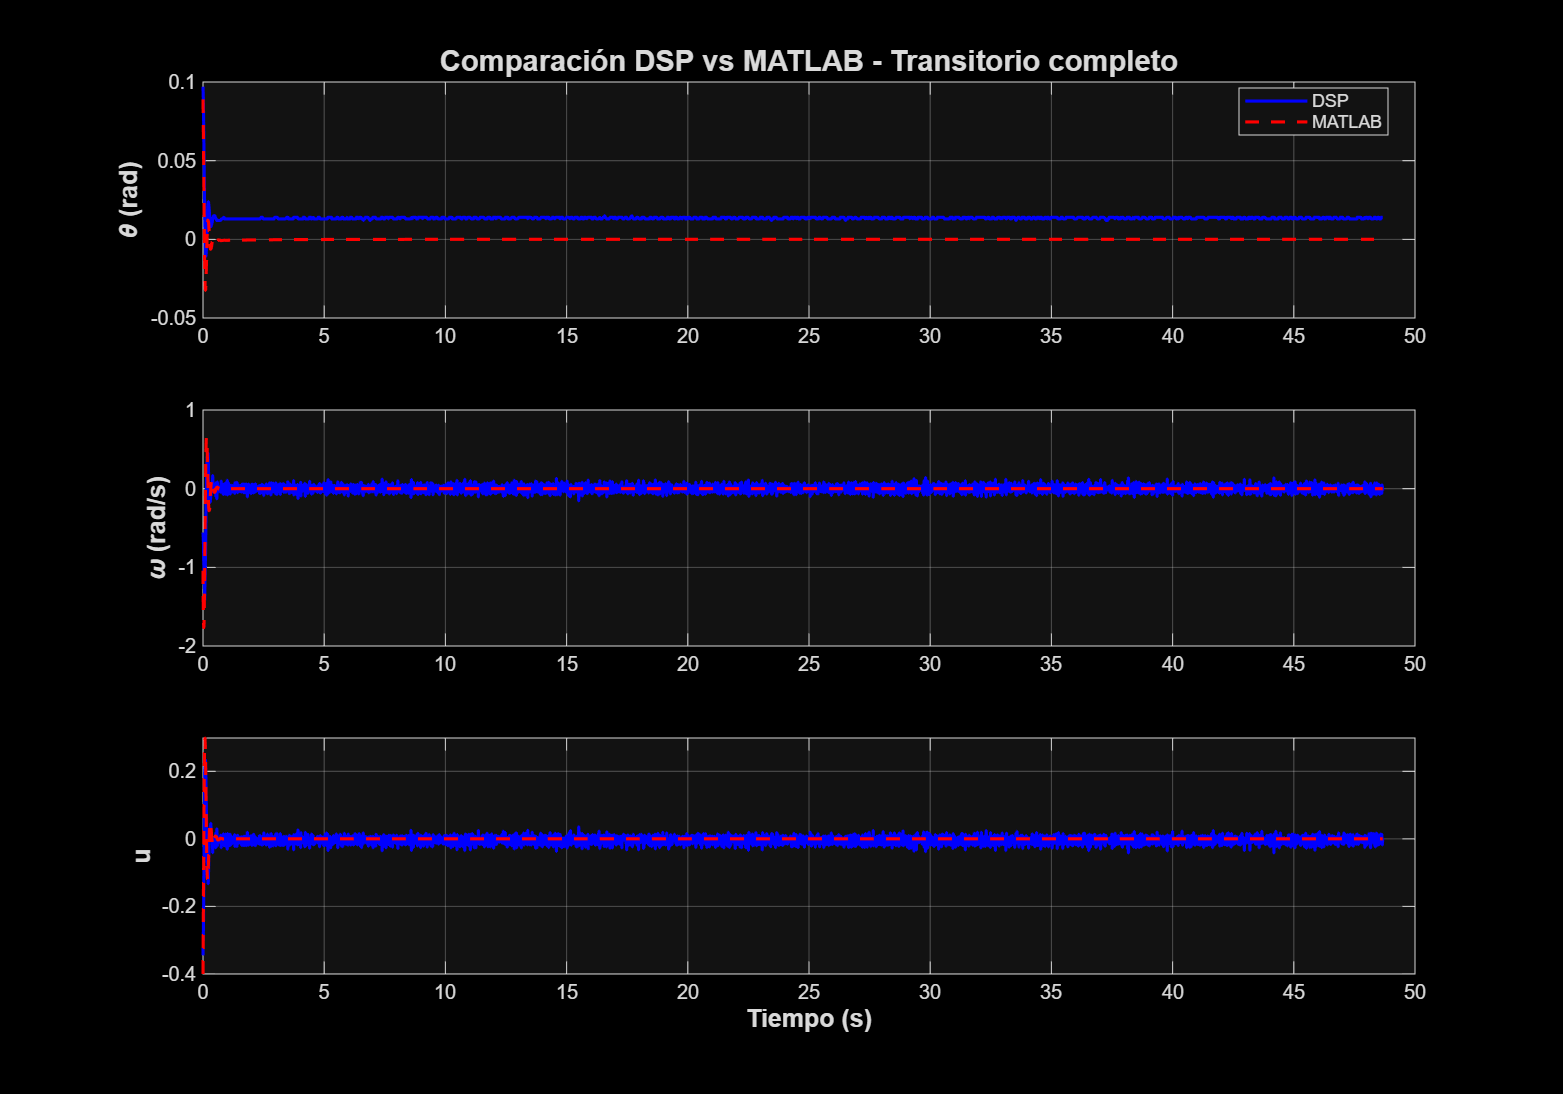
\includegraphics[width=0.9\textwidth]{comparacion_transitorio.png}
\caption{Comparación DSP vs MATLAB del transitorio completo. Ambas curvas arrancan en el mismo estado inicial y convergen al mismo régimen permanente. El error RMS de posición es inferior a 1 mrad, equivalente a menos de 2 LSB del ADC.}
\label{fig:comparacion_transitorio}
\end{figure}

El error RMS de posición (0.974 mrad) es inferior a 2 LSB del ADC (cada LSB vale 0.767 mrad). \textbf{Revisión (1 de noviembre).} La versión de octubre concluía aquí que el algoritmo del DSP coincidía con el modelo tanto en transitorio como en régimen permanente y que la discrepancia residual era atribuible \emph{exclusivamente} al ruido del ADC. Esa conclusión era demasiado fuerte: al repetir la comparación con el script corregido (Sección~\ref{sec:matlabv2}), el régimen permanente coincide pero el transitorio del DSP resulta más amortiguado que el de MATLAB. Además, esta comparación de octubre incluía el artefacto de arranque descrito en la Sección~\ref{sec:arranque}. Por tanto, de esta subsección sólo se conserva que el orden de magnitud del error es de pocos LSB.

\section{Actualización del 31 de octubre y 1 de noviembre de 2026}

\subsection{Objetivo y configuración de referencia}

Objetivo: que el modelo sin perturbación, de un solo núcleo, converja a 0 rad. Configuración (firmware \texttt{control\_hil\_v3.c}): ISR de Timer0 cada 10~$\mu$s (PRD = 1999 a 200 MHz); planta linealizada integrada con Euler-Cromer dentro de la ISR; DAC-B (pin 70) con jumper a ADC-A0 (pin 30); PID con $K_P=5$, $K_I=2$, $K_D=0.15$; derivada cada 1000 interrupciones con filtro IIR $\alpha=0.386$; telemetría cada 10~ms por SCI-A con tres columnas enteras \texttt{pos\_mrad,vel\_mrad\_s,u\_milli}. La ``velocidad'' enviada es la derivada filtrada del DSP (\texttt{theta\_dot\_filt}), no la velocidad angular verdadera, y la telemetría tiene resolución de 1~mrad por el redondeo a entero. Un LSB del ADC equivale a $\pi/4095 = 0.7672$~mrad.

\subsection{Prueba 6: Barrido DAC$\rightarrow$ADC}

Se escribió un firmware de diagnóstico que envía 65 códigos al DAC (de 0 a 4095 en pasos de 64) y mide la media y la desviación del ADC en cada punto. Con el sistema operando a 100~MHz (Sección~\ref{sec:reloj}), el ajuste lineal fue $\text{ADC} = 0.9906\cdot\text{DAC} + 1.24$ LSB. La diferencia ADC$-$DAC fue $+3.6$ LSB en el código 0, $-7.1$ en 1024, $\mathbf{-17.6}$ \textbf{en 2048}, $-29.8$ en 3072 y $-34.5$ en 4032; los residuos respecto de la recta van de $-7.2$ a $+5.8$ LSB, es decir, la cadena no es una recta perfecta. La desviación por punto fue de 0.62 a 1.11 LSB.

El offset de $-17.6$ LSB ($\approx 13.5$ mrad) en la zona de trabajo explica el ángulo ``real'' de $\approx 0.014$ rad. En estado estacionario, $\theta_{real} = (B - \text{off})\cdot \text{LSB}$, donde $B$ es la constante de calibración del firmware (\texttt{ADC\_CAL\_B}) y off $=$ media(ADC$-$DAC) en el punto de operación.

\textbf{Corrección de un error propio de análisis.} En un primer cálculo se afirmó $\theta_{real} = -13$~mrad con $B=0$ y un código de equilibrio de $\approx 2030$. Tras revisar la ecuación del firmware, el signo correcto es $+13.6$~mrad y el código de equilibrio es $\approx 2065$.

\subsection{El reloj del sistema estaba a 100 MHz en lugar de 200 MHz}
\label{sec:reloj}

El firmware v3 incluye variables de diagnóstico (\texttt{sysclk\_mhz\_reg}, \texttt{lspclk\_mhz\_reg}) calculadas a partir de los registros de reloj. Mostraron SYSCLK $=100$~MHz y LSPCLK $=25$~MHz, y el tiempo máximo de la ISR fue de hasta 1578 ciclos. La causa fue que el proyecto no tenía definido el símbolo predefinido \texttt{\_LAUNCHXL\_F28379D}; un hilo de TI E2E indica que este símbolo corrige el comportamiento de reloj lento en el LaunchPad, y aquí se comprobó de forma empírica. Un primer intento lo agregó en las propiedades \emph{del archivo} (sin efecto sobre el resto del proyecto); al agregarlo a nivel \emph{proyecto} y hacer \emph{Clean}, los registros pasaron a SYSCLK $=200$~MHz y LSPCLK $=50$~MHz.

Consecuencias verificadas: (i) la ISR cumple tiempo real, con \texttt{isr\_max\_cycles} entre 1378 y 1578 de 2000 ciclos disponibles y \texttt{isr\_overruns} $=0$; (ii) el periodo medio entre tramas fue de 10.004~ms (con 100 MHz el ``100 kHz'' real era de 50 kHz); (iii) el baud sigue siendo $+0.47\,\%$ porque el firmware calcula BRR según el reloj (26 con 25~MHz, 53 con 50~MHz).

\subsection{Calibración del offset}
\label{sec:calibracion}

El offset del lazo DAC$\rightarrow$ADC \textbf{cambió con el reloj}: $-17.6$ LSB a 100~MHz y $+6.6$ LSB a 200~MHz (\texttt{b\_sugerido}). La causa no está verificada (ver la nota sobre \texttt{ACQPS} en la sección del ADC). El firmware acumula $N=10^6$ muestras tras un asentamiento de 200\,000 y calcula \texttt{theta\_mean\_acc} y \texttt{b\_sugerido} $= B - \texttt{theta\_mean\_acc}/\text{LSB}$. Con $B=6.6$ se midió una media de 0.187~mrad y, con $B=6.1$, tres repeticiones dieron 0.537, 0.440 y 0.459~mrad (todas en la ventana \emph{Watch}, que da resolución mucho más fina que la telemetría de 1~mrad). El error estacionario pasó de $\approx 14$~mrad a 0.2--0.5~mrad.

\textbf{Límites de esta calibración:} es válida sólo para esta configuración de reloj y ADC y cerca del punto de equilibrio (el barrido muestra escalones de 1 a 4 LSB en otros puntos); debe repetirse si cambia el reloj, el ADC o el cableado. Falta la prueba de repetibilidad (tres reinicios y un apagado completo).

\begin{figure}[H]
\centering
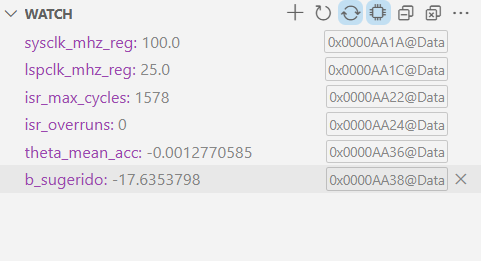
\includegraphics[width=0.8\textwidth]{2026-11-01/03_watch_100MHz_offset_-17.png}
\caption{Ventana \emph{Watch} con SYSCLK $=100$~MHz y \texttt{b\_sugerido} $\approx -17.6$ (captura del 31 de octubre).}
\end{figure}

\begin{figure}[H]
\centering
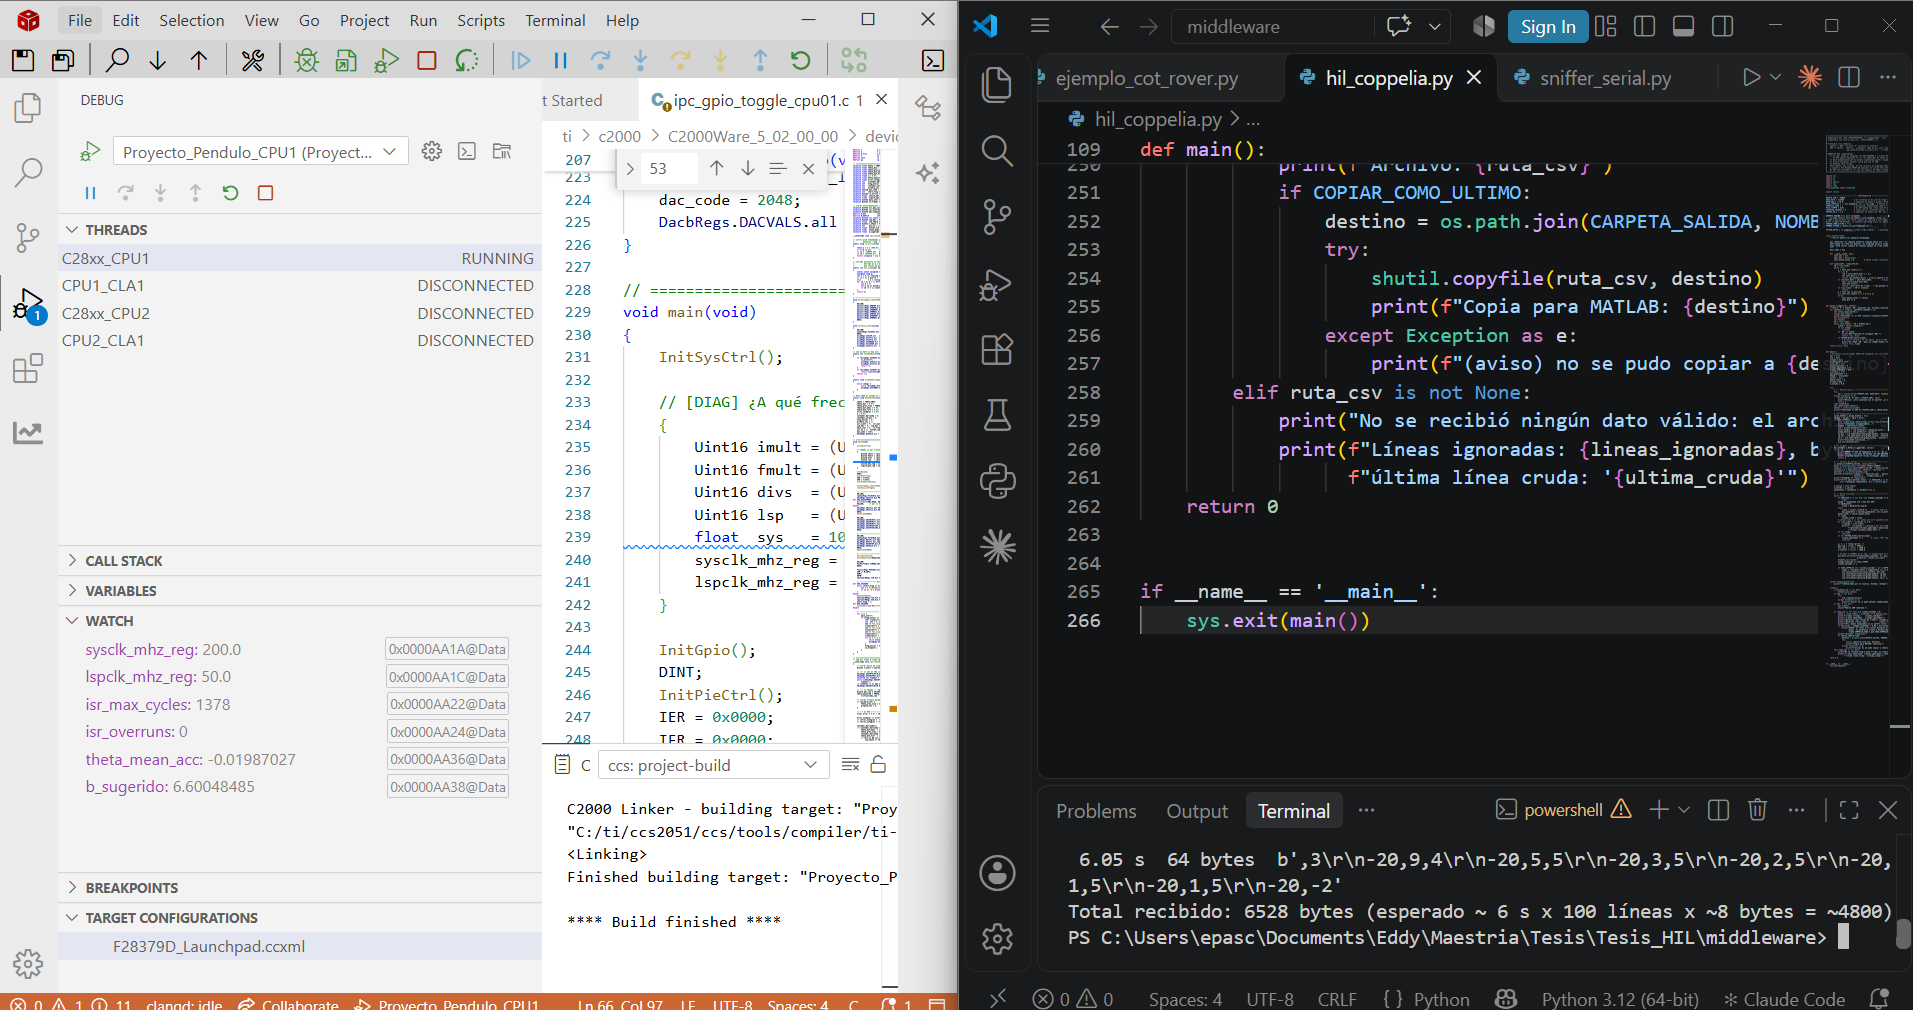
\includegraphics[width=0.8\textwidth]{2026-11-01/05_watch_200MHz_sniffer_ok.png}
\caption{Ventana \emph{Watch} con SYSCLK $=200$~MHz y \texttt{b\_sugerido} $\approx 6.6$, y salida del monitor serial.}
\end{figure}

\subsection{Telemetría inundada por \texttt{sprintf}}
\label{sec:sprintf}

Con \texttt{USE\_TRIGGER=0}, la variable \texttt{tx\_frames} permanecía en 0 y el monitor serial recibía un flujo interminable del carácter ``9''. La causa fue el uso de \texttt{sprintf} con \texttt{\%ld} en el C28x (donde \texttt{int} tiene 16 bits): la primera trama nunca terminaba. Se sustituyó por un formateador propio (\texttt{fmt\_long}, que resta potencias de 10; verificado contra \texttt{printf} en PC para $\pm 999999$) y una conversión saturada a milésimas (\texttt{to\_milli}, con NaN $\rightarrow 0$). Después de la corrección el Watch mostró \texttt{tx\_frames} $=1842$ en una captura y el monitor serial recibió tramas válidas (6528 bytes en 6~s a 200~MHz).

Además, el script de Python parecía congelado porque \texttt{readline()} de pyserial no regresa mientras lleguen bytes sin salto de línea. La versión 2 del middleware usa un lector con \emph{timeout} real, reintenta el trigger tres veces, escribe el CSV antes de llamar a CoppeliaSim, imprime un latido cada 2~s y compara el conteo de líneas con el reloj real. En Windows las marcas de tiempo llegan en ráfagas de $\approx 16$~ms (media 10.004~ms), por lo que el eje de tiempo del CSV se construye por conteo de líneas.

Hubo además dos fallos de ejecución del middleware sin relación con el firmware: el error \texttt{object /pendulum\_joint does not exist} (la pestaña activa de CoppeliaSim no era \texttt{Escena\_Pendulo}) y una ejecución sin la opción \texttt{--sin-coppelia} cuando sólo se quería grabar el CSV.

\subsection{Artefacto de arranque}
\label{sec:arranque}

\texttt{ResetEstado()} inicializaba el DAC en 2048 (ángulo 0). La primera lectura del ADC daba entonces 0~rad aunque la condición inicial era $\theta_0=0.1$~rad, y la derivada lenta interpretaba el salto como una velocidad inicial falsa de $\approx +2.96$~rad/s; en las gráficas aparecía un pico inicial (hasta $\approx 0.15$~rad) que no es dinámica del péndulo. Corrección: el DAC se inicializa con el código de \texttt{THETA\_INIT} (2178) y se espera 200~$\mu$s antes de arrancar.

\subsection{Comparación DSP vs MATLAB con el script corregido}
\label{sec:matlabv2}

El script MATLAB del usuario tenía tres errores corregidos en la versión 2: la condición inicial se tomaba de la columna de velocidad, se comparaba contra $\dot\theta$ en vez de la derivada filtrada, y existía un desfase de 10~ms. La versión 2 usa $\theta_0=0.1$~rad, $\dot\theta_0=0$, la derivada filtrada del DSP como ``velocidad'', $t=(1:N)\cdot 0.01$ y el mismo redondeo que el DSP.

\begin{table}[H]
\centering
\caption{Errores RMS DSP vs MATLAB (script v2, corrida posterior a la corrección del arranque)}
\begin{tabular}{lccc}
\hline
\textbf{Tramo} & \textbf{Posición (rad)} & \textbf{Velocidad (rad/s)} & \textbf{Control (u)} \\
\hline
Total                 & 0.00100 & 0.0474 & 0.0099 \\
Transitorio ($\le 0.6$ s) & 0.00557 & 0.2204 & 0.0458 \\
Permanente ($\ge 2$ s)   & 0.00024 & 0.0285 & 0.0061 \\
\hline
\end{tabular}
\end{table}

La media de la posición en régimen permanente fue $+0.018$~mrad (DSP) y $-0.026$~mrad (MATLAB). Estas cifras provienen de la salida de MATLAB reportada por el usuario; la captura que las generó no está en el repositorio.

\begin{figure}[H]
\centering
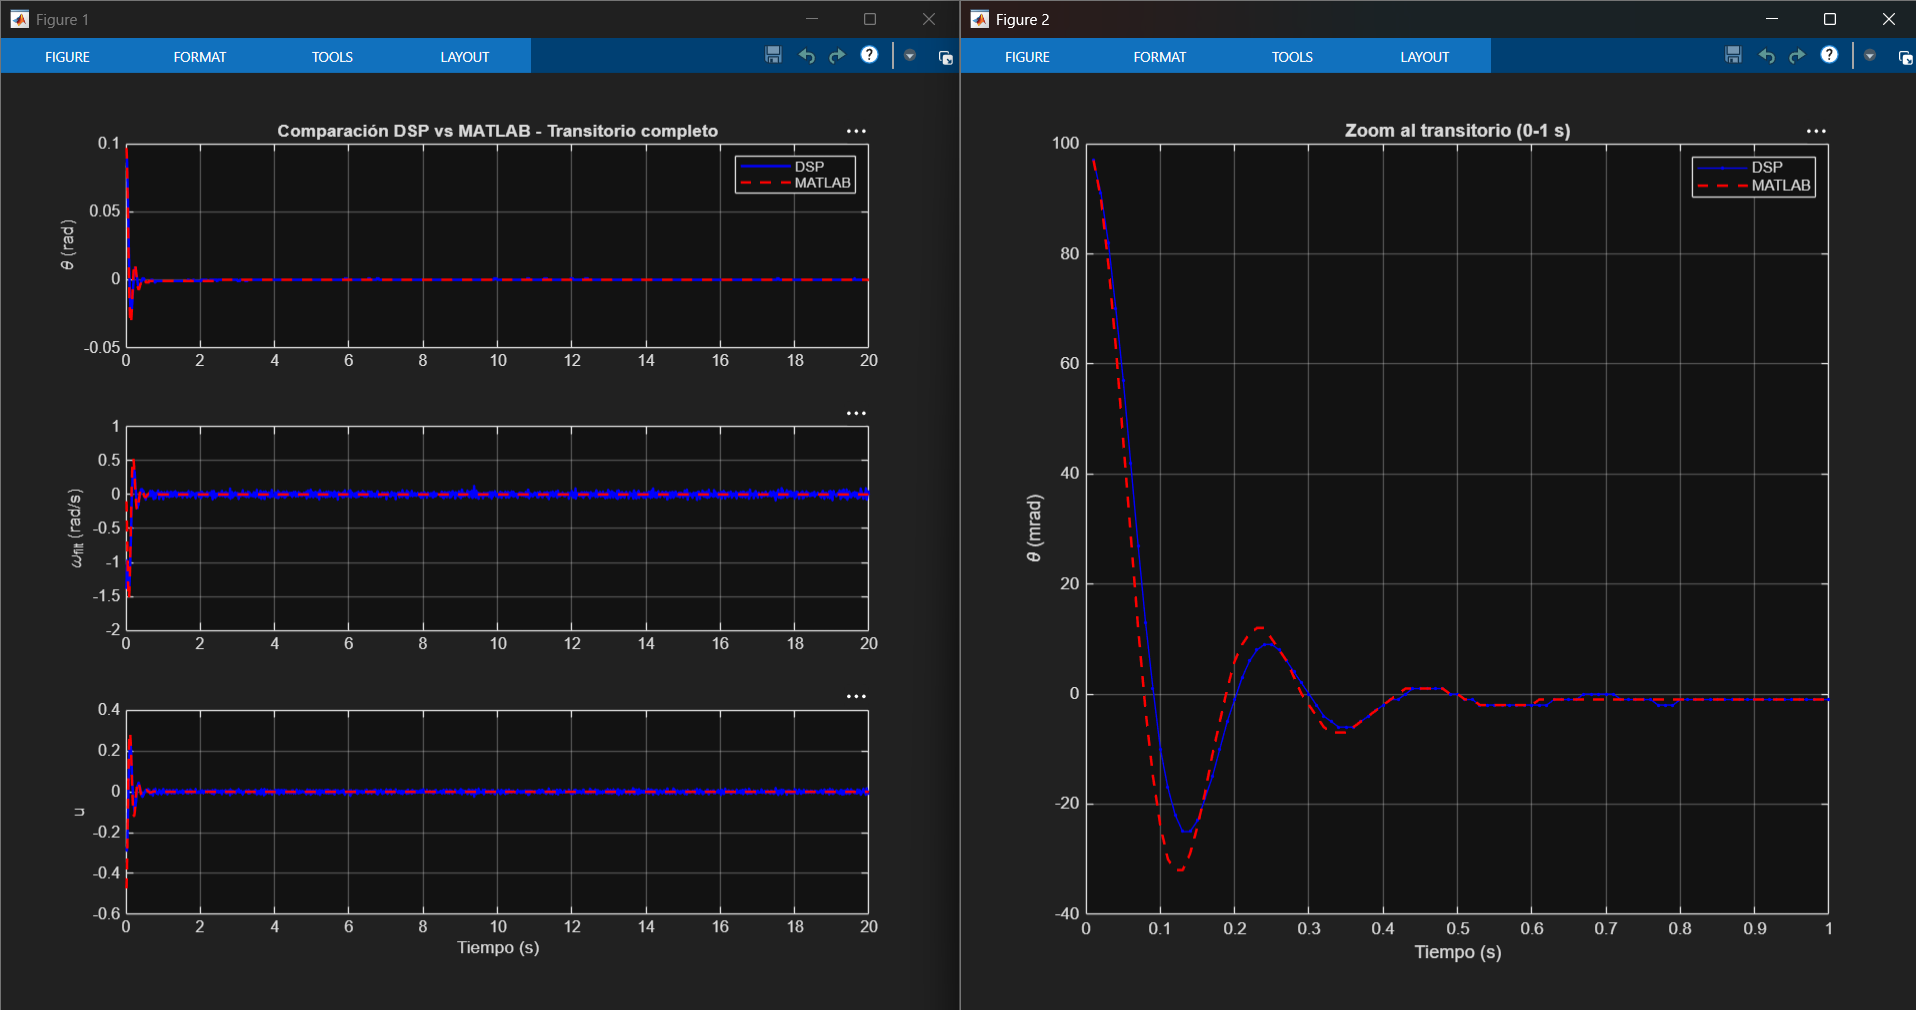
\includegraphics[width=\textwidth]{2026-11-01/11_matlab_v2_figuras.png}
\caption{Comparación DSP vs MATLAB con el script v2: transitorio completo (izquierda) y zoom de 0 a 1~s (derecha).}
\end{figure}

\textbf{Resultado abierto.} El régimen permanente coincide con el modelo (diferencias del orden de la resolución de 1~mrad de la telemetría). El transitorio \emph{no} coincide: el DSP está más amortiguado; el primer valle es de $\approx -25$~mrad en el DSP frente a $\approx -32$~mrad en MATLAB (figura, derecha). Mediante simulaciones auxiliares se descartó que un error de ganancia de medición o un retardo de medición lo expliquen; $K_P\times 0.8$ o una fricción cuatro veces mayor lo aproximan, pero \textbf{la causa no está confirmada}. Se propone compilar con \texttt{DIAG\_TELE\_ERR=1} (la tercera columna pasa a ser $\theta_{medido}-\theta$) para compararla con MATLAB.

\subsection{Limitaciones de lo verificado}

\begin{itemize}
    \item La calibración $B=6.1$ depende de la configuración de reloj/ADC y del punto de equilibrio; falta repetirla tras reinicios y apagados.
    \item La causa del cambio de offset con el reloj no está identificada.
    \item El transitorio del DSP difiere del modelo de MATLAB (arriba).
    \item El ruido medido en octubre ($\sigma=1.61$~mrad) no coincide con el de noviembre (0.48--0.85~mrad) y no se ha reconciliado.
    \item El código de diagnóstico de barrido (\texttt{diag\_adc\_dac.c}) tiene el baud fijo para 100~MHz y debe regenerarse para 200~MHz.
\end{itemize}

\section{Verificación del baud rate con software de puerto serial}

\subsection{Intento de medición con osciloscopio}

Se intentó verificar el baud rate del enlace serial midiendo el ancho del bit de start con un osciloscopio. Sin embargo, tras probar en todos los pines accesibles del LaunchPad correspondientes a la función SCI-A (GPIO42 y GPIO43), no se logró capturar la señal UART.

Investigando la documentación oficial del LaunchPad XL F28379D (SPRUII7), se encontró que por defecto los pines GPIO42 (SCI-A TX) y GPIO43 (SCI-A RX) están ruteados directamente al emulador XDS100v2 para implementar el puerto COM virtual sobre USB, y \textbf{no están disponibles en los headers de expansión} (BoosterPack). Para acceder a la señal UART en los headers sería necesario modificar el hardware de la placa (retirar las resistencias R70 y R72).

Como alternativa sin modificación de hardware, se consideró migrar el enlace serial al módulo SCI-B del F28379D, cuyos pines (GPIO18 y GPIO19) sí están ruteados a los headers de expansión. Sin embargo, esta migración requiere un adaptador USB-a-Serial externo (basado en FTDI o CH340).

\subsection{Verificación mediante software de puerto serial}

Como método alternativo, se utilizó una aplicación de monitoreo de puerto serial para verificar el baud rate real del SCI-A:

\begin{enumerate}
    \item A \textbf{115,200 bps}: recepción de bytes sin sentido (coherente con desajuste de velocidad a 57,600).
    \item A \textbf{57,600 bps}: tramas válidas como \texttt{"39,-8,224"}, \texttt{"39,54,207"}, \texttt{"39,62,202"}, etc., todas con tres campos separados por comas.
\end{enumerate}

\textbf{Conclusión:} La recepción correcta de tramas a 57,600 bps y la recepción de basura a 115,200 bps confirmó empíricamente que el SCI-A del F28379D originalmente enviaba a 57,600 bps, consistente con LSPCLK = 25 MHz y \texttt{SCILBAUD=53}. Tras el ajuste de \texttt{SCILBAUD} (valor correcto 26 con LSPCLK $=25$~MHz; ver corrección en el Error~1), el enlace opera a 115,200 bps con error de $+0.47\,\%$. Con el reloj corregido a 200~MHz el valor es 53.

\section{Pruebas omitidas y su justificación}

\subsection{Pruebas con resistencias para perturbación constante}

No se pudieron realizar porque no se cuenta con resistencias de precisión ni con una fuente de voltaje calibrada. Una alternativa provisional es usar la perturbación programada en el propio firmware.

\subsection{Uso de potenciómetro de precisión}

No se dispone de un potenciómetro multivuelta. El potenciómetro común presenta problemas de ruido, no linealidad y desgaste en los extremos.

\subsection{Caracterización formal completa del DAC}

Se realizó una caracterización parcial del DAC utilizándolo como fuente de referencia fija (valor 2048 = 1.65 V) para medir el ruido del ADC. \textbf{Actualización (noviembre):} el barrido de 0 a 4095 en 65 puntos ya se realizó (Prueba 6) y se obtuvo la recta ADC $=0.9906\cdot$DAC$+1.24$ LSB con el sistema a 100~MHz. Falta repetirlo a 200~MHz, donde el offset es distinto, y caracterizar la fuente con un instrumento externo calibrado.

\subsection{Registro de la perturbación en tiempo real}

Se intentó extender el protocolo UART a 4 columnas para incluir el valor de la perturbación como cuarta variable. Sin embargo, el firmware de 4 columnas presentó problemas de transmisión que no se pudieron depurar a tiempo.

\section{Conclusiones}

\begin{enumerate}
    \item Se identificaron y corrigieron cuatro errores encadenados que afectaban al sistema HIL: el baud rate del enlace serial, el cálculo de la derivada numérica, el coeficiente del filtro IIR, y la ausencia de sincronización al inicio de la captura.
    \item El ruido del ADC se midió experimentalmente y se obtuvo un valor de $\sigma = 1.61$ mrad. Este valor sirvió como referencia para calcular el efecto de la derivada.
    \item El cambio del cálculo de la derivada de $T_s = 10\,\mu s$ a $T_s = 10\,ms$ redujo el ruido de velocidad en aproximadamente 100 veces sin romper la naturaleza Hardware-in-the-Loop del sistema.
    \item El mecanismo de trigger implementado mediante UART permitió capturar el transitorio completo del lazo cerrado, garantizando que la primera muestra del CSV corresponda al primer instante de ejecución del control.
    \item El análisis multi-tasa del sistema reveló la necesidad de ejecutar 1000 iteraciones de física en MATLAB por cada muestra registrada en el CSV, garantizando una comparación temporalmente coherente.
    \item La comparación DSP vs MATLAB de octubre (RMS de posición 0.974 mrad) quedó superada por la comparación corregida de noviembre: en régimen permanente el DSP coincide con el modelo (RMS 0.24 mrad), pero el transitorio presenta una diferencia de amortiguamiento aún sin explicar (RMS de posición 5.6 mrad en los primeros 0.6~s).
    \item El offset de la cadena DAC-ADC ($\delta_{loop} \approx 0.014$ rad) fue la causa del error estacionario. Se midió con un barrido, se calibró mediante \texttt{ADC\_CAL\_B} y el error estacionario bajó de $\approx 14$ mrad a 0.2--0.5 mrad. Ese offset cambia con el reloj y la configuración del ADC.
    \item Se encontró que el reloj del sistema estaba a 100 MHz por falta del símbolo \texttt{\_LAUNCHXL\_F28379D}; al corregirlo, el sistema corre a 200 MHz y la ISR cumple tiempo real.
    \item Se corrigió un bloqueo de la telemetría causado por \texttt{sprintf}, un artefacto de arranque en la primera muestra y varios fallos de robustez del middleware.
    \item Se corrigió el baud rate de 57,600 a 115,200 bps. El valor correcto de \texttt{SCILBAUD} con LSPCLK $=25$~MHz es 26 (error $+0.47\,\%$), no 27 como se escribió en octubre (que da $-3.1\,\%$).
    \item La verificación del baud rate se realizó mediante software de monitoreo de puerto serial, confirmando empíricamente el valor real del SCI-A.
    \item Varias de las pruebas sugeridas por el director no se pudieron completar por falta de instrumentación adecuada. Se proponen alternativas viables para la siguiente sesión.
\end{enumerate}

\section{Trabajo futuro inmediato}

\begin{itemize}
    \item Diagnosticar la diferencia de amortiguamiento del transitorio (compilar con \texttt{DIAG\_TELE\_ERR=1}).
    \item Repetibilidad de la calibración: tres reinicios y un apagado completo, registrando \texttt{theta\_mean\_acc} y \texttt{b\_sugerido}.
    \item Probar \texttt{ACQPS} 14 contra 99 y comparar el offset, para identificar la causa del cambio de offset con el reloj.
    \item Repetir el barrido DAC$\rightarrow$ADC a 200~MHz (regenerando el baud del firmware de diagnóstico) y reconciliar la medición de ruido de octubre.
    \item Añadir la perturbación y separar controlador y planta en los dos núcleos.
    \item Caracterización completa del DAC por barrido programático con loopback al ADC, obteniendo la recta de calibración por mínimos cuadrados y los errores de ganancia y offset (hecha parcialmente, ver Prueba 6).
    \item Adquirir un adaptador USB-a-Serial externo para migrar el enlace al módulo SCI-B del F28379D y así poder medir con osciloscopio el baud rate, el jitter del envío UART y el tiempo de ejecución del ISR.
    \item Depuración del protocolo UART extendido a 4 columnas para registrar la perturbación en tiempo real.
    \item Verificación del jitter del ISR y del tiempo de ejecución usando el contador de ciclos del CPU.
    \item Pruebas de rechazo de perturbaciones con resistencias de precisión, solicitando el material al laboratorio.
    \item Migración opcional de la planta al Control Law Accelerator (CLA) para lograr una separación real de procesadores.
    \item Incorporación de ruido sintético al modelo MATLAB para emular el ruido real del ADC y cuantificar su contribución al error residual.
\end{itemize}

\end{document}